\documentclass[tikz,border=25pt]{standalone}
\usepackage[utf8]{inputenc}
\usepackage[T1]{fontenc}
\usepackage{amsmath,amssymb}

\usetikzlibrary{
  arrows.meta,
  positioning,
  shapes.geometric,
  shapes.misc,
  calc,
  fit,
  backgrounds
}

% Clean modern sans-serif typography
\renewcommand{\familydefault}{\sfdefault}

% ---------------------------------------------------------------------------
% Custom Color Palette (Physics-grounded, high contrast, non-generic)
% ---------------------------------------------------------------------------
\definecolor{headerNavy}{HTML}{0F172A}
\definecolor{headerBlue}{HTML}{1E3A8A}
\definecolor{frameBorder}{HTML}{94A3B8}
\definecolor{frameBg}{HTML}{F8FAFC}

% Neutral / Gateway Nodes
\definecolor{gateBg}{HTML}{FFFFFF}
\definecolor{gateBorder}{HTML}{334155}
\definecolor{gateText}{HTML}{0F172A}

% Outcome Colors (Strictly consistent across all branches)
% Green: Secure / Normal / High / None
\definecolor{secureBg}{HTML}{ECFDF5}
\definecolor{secureBorder}{HTML}{059669}
\definecolor{secureText}{HTML}{065F46}

% Amber: Warning / Degraded / Alert
\definecolor{warnBg}{HTML}{FFFBEB}
\definecolor{warnBorder}{HTML}{D97706}
\definecolor{warnText}{HTML}{92400E}

% Red: Compromised / Anomalous / Critical / Abort / Early Reject
\definecolor{dangerBg}{HTML}{FEF2F2}
\definecolor{dangerBorder}{HTML}{DC2626}
\definecolor{dangerText}{HTML}{991B1B}

% Cyan: Ingestion / Processing
\definecolor{procBg}{HTML}{F0F9FF}
\definecolor{procBorder}{HTML}{0284C7}
\definecolor{procText}{HTML}{0369A1}

% Violet: Audit Ledger
\definecolor{ledgerBg}{HTML}{F5F3FF}
\definecolor{ledgerBorder}{HTML}{7C3AED}
\definecolor{ledgerText}{HTML}{5B21B6}

% Gold: Math callout
\definecolor{mathBg}{HTML}{FEFCE8}
\definecolor{mathBorder}{HTML}{CA8A04}
\definecolor{mathText}{HTML}{713F12}

\begin{document}
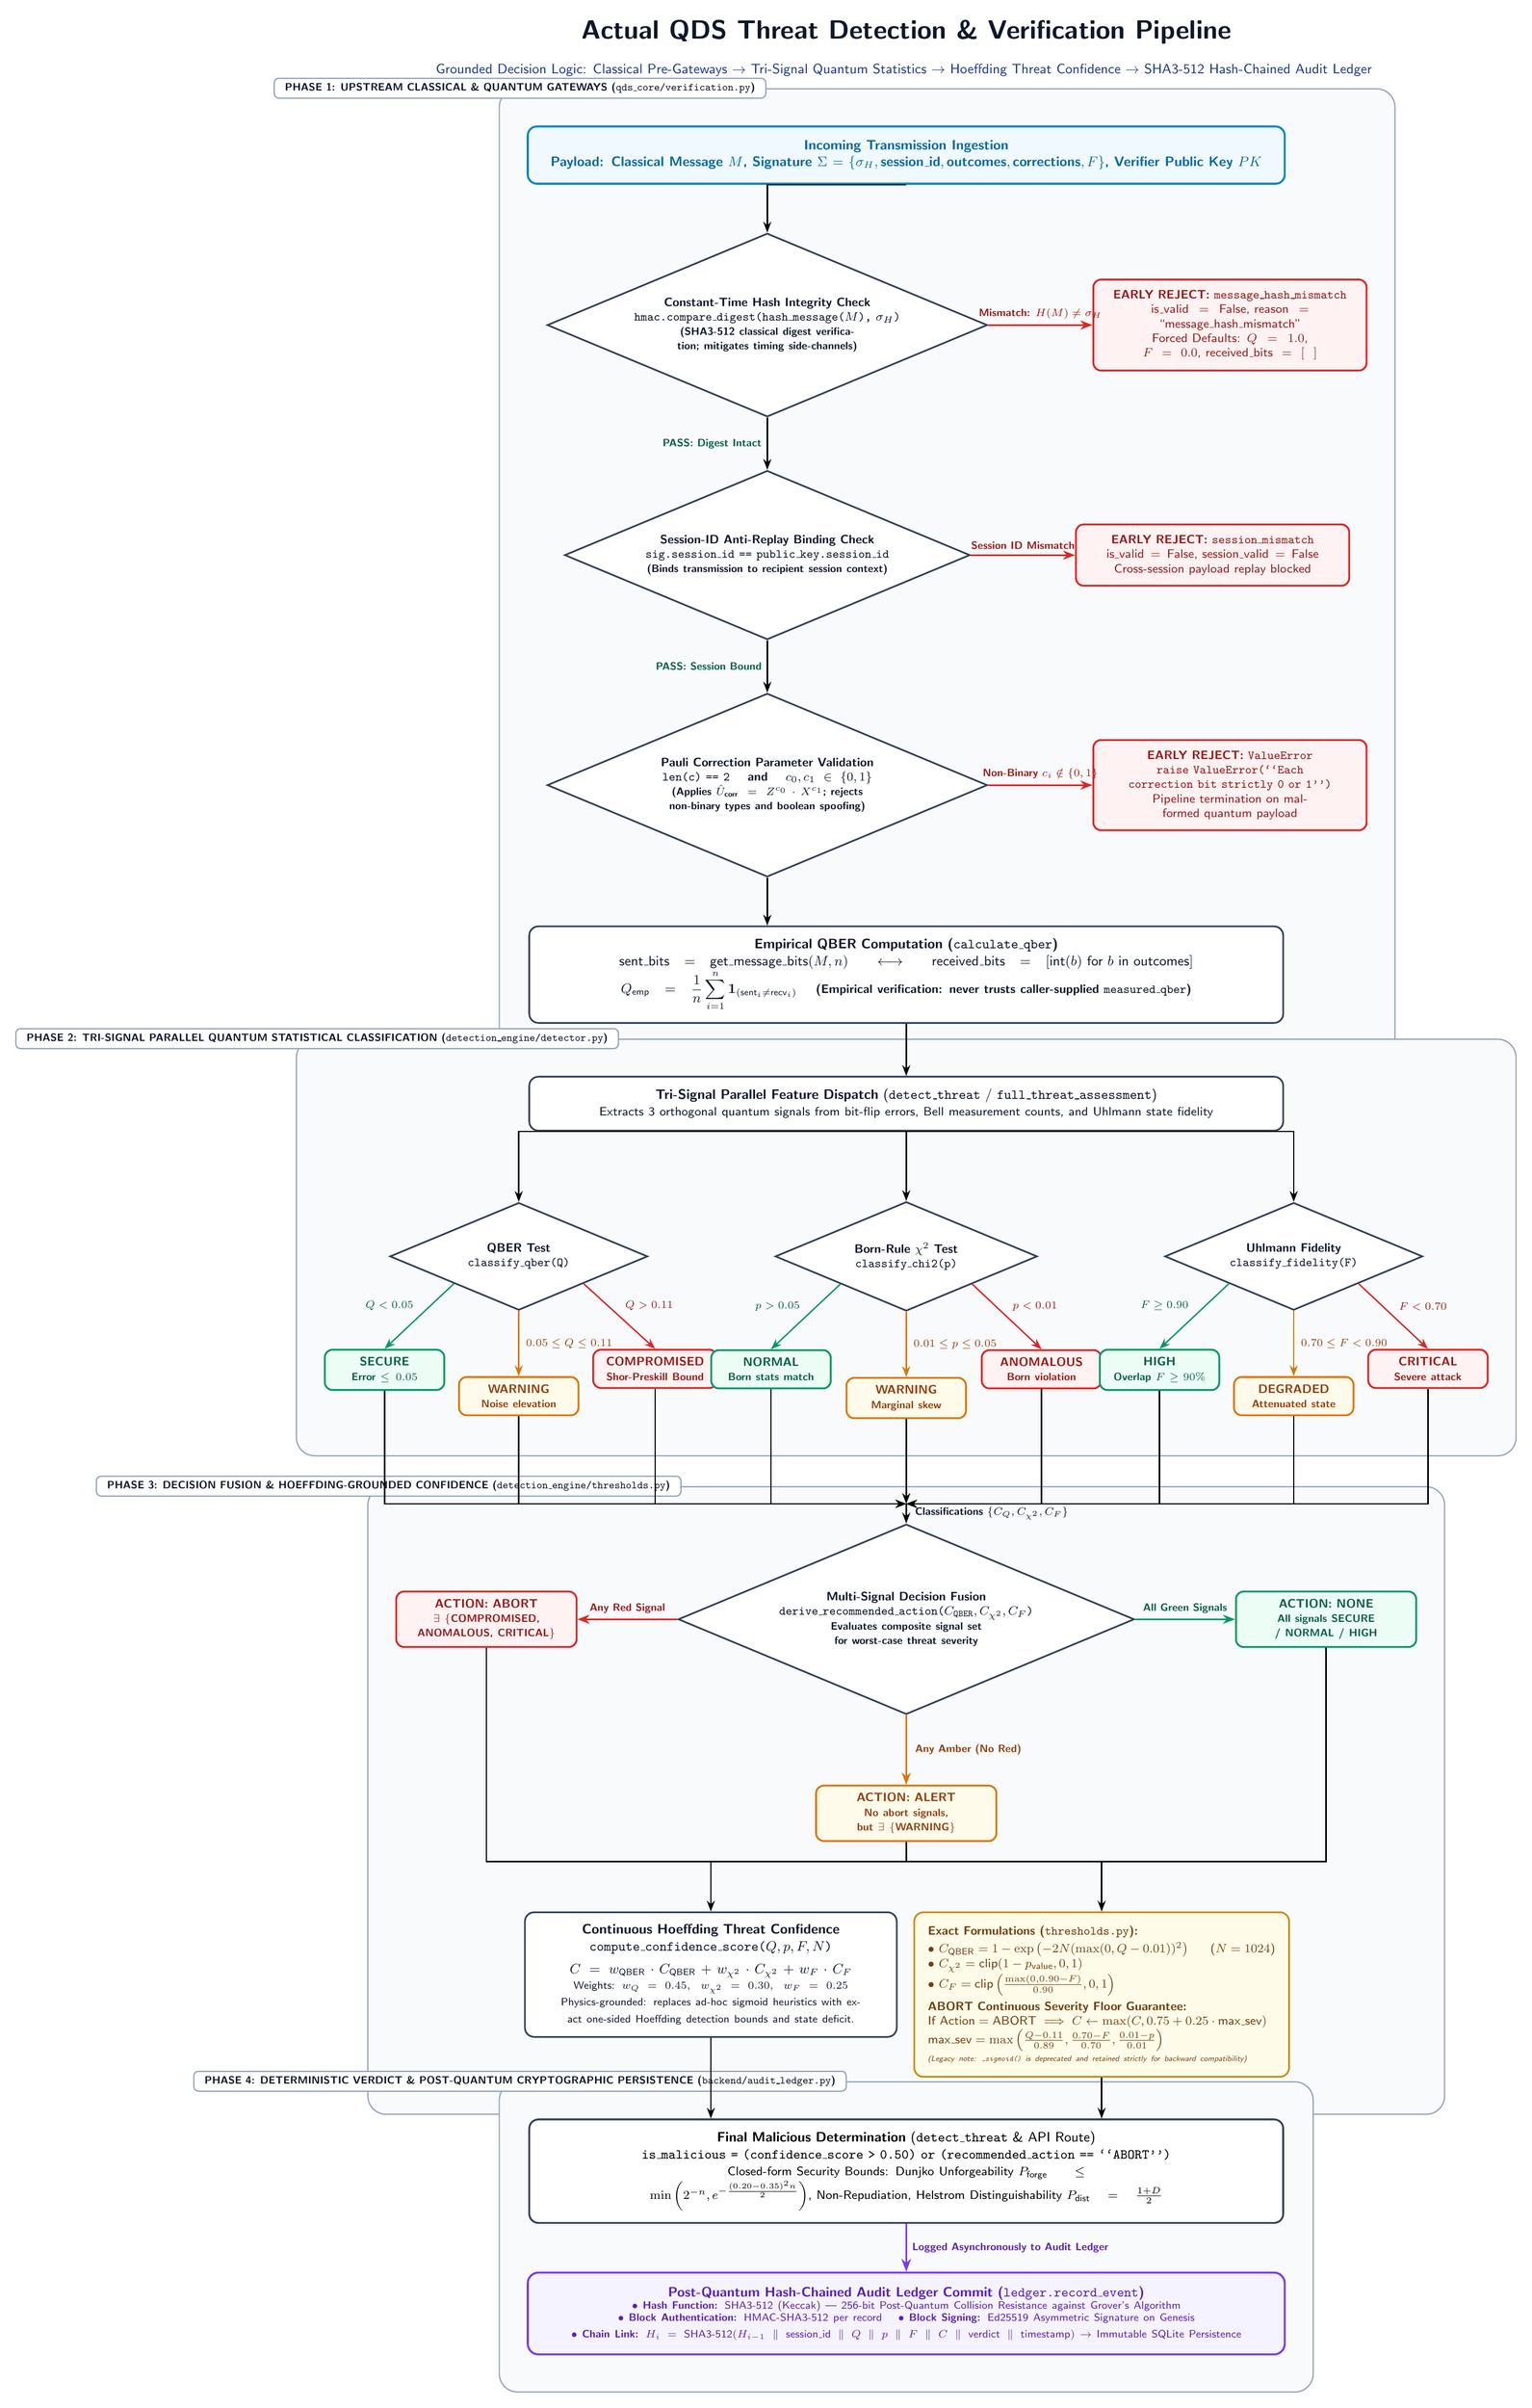
\begin{tikzpicture}[
  font=\small,
  >=Stealth,
  line width=0.9pt,
  % Node Styles with explicit text widths for clean wrapping
  titleNode/.style={
    align=center,
    font=\bfseries\LARGE,
    text=headerNavy
  },
  subTitleNode/.style={
    align=center,
    font=\small,
    text=headerBlue
  },
  processStep/.style={
    draw=gateBorder,
    fill=gateBg,
    rounded corners=6pt,
    align=center,
    line width=1.1pt,
    inner sep=8pt,
    text=gateText,
    font=\small
  },
  entryStep/.style={
    draw=procBorder,
    fill=procBg,
    rounded corners=6pt,
    align=center,
    line width=1.3pt,
    inner sep=9pt,
    text=procText,
    font=\small\bfseries
  },
  decisionDiamond/.style={
    diamond,
    draw=gateBorder,
    fill=gateBg,
    aspect=2.4,
    align=center,
    line width=1.1pt,
    inner sep=3pt,
    text=gateText,
    font=\footnotesize\bfseries
  },
  earlyRejectNode/.style={
    draw=dangerBorder,
    fill=dangerBg,
    rounded corners=5pt,
    align=center,
    line width=1.2pt,
    inner sep=7pt,
    text=dangerText,
    font=\footnotesize
  },
  statusSecure/.style={
    draw=secureBorder,
    fill=secureBg,
    rounded corners=5pt,
    align=center,
    line width=1.2pt,
    inner sep=5pt,
    text=secureText,
    font=\footnotesize\bfseries
  },
  statusWarn/.style={
    draw=warnBorder,
    fill=warnBg,
    rounded corners=5pt,
    align=center,
    line width=1.2pt,
    inner sep=5pt,
    text=warnText,
    font=\footnotesize\bfseries
  },
  statusDanger/.style={
    draw=dangerBorder,
    fill=dangerBg,
    rounded corners=5pt,
    align=center,
    line width=1.2pt,
    inner sep=5pt,
    text=dangerText,
    font=\footnotesize\bfseries
  },
  actionBox/.style={
    draw=gateBorder,
    fill=gateBg,
    rounded corners=6pt,
    align=center,
    line width=1.2pt,
    inner sep=8pt,
    font=\small
  },
  ledgerBox/.style={
    draw=ledgerBorder,
    fill=ledgerBg,
    rounded corners=7pt,
    align=center,
    line width=1.3pt,
    inner sep=9pt,
    text=ledgerText,
    font=\small
  },
  mathCallout/.style={
    draw=mathBorder,
    fill=mathBg,
    rounded corners=6pt,
    align=left,
    line width=1.1pt,
    inner sep=9pt,
    text=mathText,
    font=\footnotesize
  },
  groupLabel/.style={
    font=\bfseries\scriptsize,
    text=headerNavy,
    fill=white,
    draw=frameBorder,
    line width=0.8pt,
    inner xsep=7pt,
    inner ysep=3pt,
    rounded corners=3pt
  }
]

% ===========================================================================
% TITLE HEADER
% ===========================================================================
\node[titleNode] (title) at (0, 0) {Actual QDS Threat Detection \& Verification Pipeline};
\node[subTitleNode, below=0.2cm of title] (subtitle) {
  Grounded Decision Logic: Classical Pre-Gateways $\to$ Tri-Signal Quantum Statistics $\to$ Hoeffding Threat Confidence $\to$ SHA3-512 Hash-Chained Audit Ledger
};

% ===========================================================================
% ZONE 1: INGESTION & UPSTREAM VERIFICATION GATEWAYS (qds_core/verification.py)
% ===========================================================================
\node[entryStep, below=1.0cm of subtitle, text width=16.8cm] (inputNode) {
  \textbf{Incoming Transmission Ingestion} \\
  Payload: Classical Message $M$, Signature $\Sigma = \{\sigma_H, \text{session\_id}, \text{outcomes}, \text{corrections}, F\}$, Verifier Public Key $PK$
};

% Gate 1: Constant-Time Hash Integrity Check
\node[decisionDiamond, below=1.1cm of inputNode, xshift=-3.2cm, text width=6.4cm] (hashGate) {
  \textbf{Constant-Time Hash Integrity Check} \\
  \texttt{hmac.compare\_digest(hash\_message($M$), $\sigma_H$)} \\
  \scriptsize (SHA3-512 classical digest verification; mitigates timing side-channels)
};

\node[earlyRejectNode, right=2.4cm of hashGate, text width=5.8cm] (hashReject) {
  \textbf{EARLY REJECT: \texttt{message\_hash\_mismatch}} \\
  $\text{is\_valid} = \text{False}$, $\text{reason} = \text{``message\_hash\_mismatch''}$ \\
  Forced Defaults: $Q = 1.0$, $F = 0.0$, $\text{received\_bits} = [\;]$
};

% Gate 2: Session-ID Binding Check
\node[decisionDiamond, below=1.2cm of hashGate, text width=6.4cm] (sessionGate) {
  \textbf{Session-ID Anti-Replay Binding Check} \\
  \texttt{sig.session\_id == public\_key.session\_id} \\
  \scriptsize (Binds transmission to recipient session context)
};

\node[earlyRejectNode, right=2.4cm of sessionGate, text width=5.8cm] (sessionReject) {
  \textbf{EARLY REJECT: \texttt{session\_mismatch}} \\
  $\text{is\_valid} = \text{False}$, $\text{session\_valid} = \text{False}$ \\
  Cross-session payload replay blocked
};

% Gate 3: Pauli Correction Bit Validation
\node[decisionDiamond, below=1.2cm of sessionGate, text width=6.4cm] (pauliGate) {
  \textbf{Pauli Correction Parameter Validation} \\
  \texttt{len(c) == 2} \quad and \quad $c_0, c_1 \in \{0, 1\}$ \\
  \scriptsize (Applies $\hat{U}_{\text{corr}} = Z^{c_0} \cdot X^{c_1}$; rejects non-binary types and boolean spoofing)
};

\node[earlyRejectNode, right=2.4cm of pauliGate, text width=5.8cm] (pauliReject) {
  \textbf{EARLY REJECT: \texttt{ValueError}} \\
  \texttt{raise ValueError(``Each correction bit strictly 0 or 1'')} \\
  Pipeline termination on malformed quantum payload
};

% Step 4: Empirical QBER Computation
\node[processStep, below=1.1cm of pauliGate, xshift=3.2cm, text width=16.8cm] (empiricalQber) {
  \textbf{Empirical QBER Computation (\texttt{calculate\_qber})} \\
  $\text{sent\_bits} = \text{get\_message\_bits}(M, n) \quad\longleftrightarrow\quad \text{received\_bits} = [\text{int}(b) \text{ for } b \text{ in outcomes}]$ \\
  $\displaystyle Q_{\text{emp}} = \frac{1}{n}\sum_{i=1}^n \mathbf{1}_{(\text{sent}_i \ne \text{recv}_i)}$ \quad \footnotesize\textbf{(Empirical verification: never trusts caller-supplied \texttt{measured\_qber})}
};

% ===========================================================================
% ZONE 2: TRI-SIGNAL PARALLEL QUANTUM DECISION PIPELINE (detection_engine/detector.py)
% ===========================================================================

% Split Coordinator
\node[processStep, below=1.2cm of empiricalQber, text width=16.8cm] (triSplit) {
  \textbf{Tri-Signal Parallel Feature Dispatch} (\texttt{detect\_threat} / \texttt{full\_threat\_assessment}) \\
  \footnotesize Extracts 3 orthogonal quantum signals from bit-flip errors, Bell measurement counts, and Uhlmann state fidelity
};

% Center diamond first: Born Rule Chi2
\node[decisionDiamond, below=1.6cm of triSplit, text width=3.8cm] (chiDiamond) {
  \textbf{Born-Rule $\chi^2$ Test} \\
  \texttt{classify\_chi2(p)}
};

% Left diamond: QBER
\node[decisionDiamond, left=2.9cm of chiDiamond, text width=3.8cm] (qberDiamond) {
  \textbf{QBER Test} \\
  \texttt{classify\_qber(Q)}
};

% Right diamond: Fidelity
\node[decisionDiamond, right=2.9cm of chiDiamond, text width=3.8cm] (fidDiamond) {
  \textbf{Uhlmann Fidelity} \\
  \texttt{classify\_fidelity(F)}
};

% --- Column 1: QBER Branches (Left) ---
\node[statusSecure, below left=1.5cm and 0.2cm of qberDiamond, text width=2.4cm] (qberSecure) {
  \textbf{SECURE} \\
  \scriptsize Error $\le 0.05$
};
\node[statusWarn, below=1.5cm of qberDiamond, text width=2.4cm] (qberWarn) {
  \textbf{WARNING} \\
  \scriptsize Noise elevation
};
\node[statusDanger, below right=1.5cm and 0.2cm of qberDiamond, text width=2.5cm] (qberDanger) {
  \textbf{COMPROMISED} \\
  \scriptsize Shor-Preskill Bound
};

% --- Column 2: Chi2 Branches (Center) ---
\node[statusSecure, below left=1.5cm and 0.2cm of chiDiamond, text width=2.4cm] (chiNormal) {
  \textbf{NORMAL} \\
  \scriptsize Born stats match
};
\node[statusWarn, below=1.5cm of chiDiamond, text width=2.4cm] (chiWarn) {
  \textbf{WARNING} \\
  \scriptsize Marginal skew
};
\node[statusDanger, below right=1.5cm and 0.2cm of chiDiamond, text width=2.4cm] (chiDanger) {
  \textbf{ANOMALOUS} \\
  \scriptsize Born violation
};

% --- Column 3: Fidelity Branches (Right) ---
\node[statusSecure, below left=1.5cm and 0.2cm of fidDiamond, text width=2.4cm] (fidHigh) {
  \textbf{HIGH} \\
  \scriptsize Overlap $F \ge 90\%$
};
\node[statusWarn, below=1.5cm of fidDiamond, text width=2.4cm] (fidDegraded) {
  \textbf{DEGRADED} \\
  \scriptsize Attenuated state
};
\node[statusDanger, below right=1.5cm and 0.2cm of fidDiamond, text width=2.4cm] (fidCritical) {
  \textbf{CRITICAL} \\
  \scriptsize Severe attack
};

% ===========================================================================
% ZONE 3: DECISION FUSION & CONFIDENCE SCORE SYNTHESIS
% ===========================================================================

\node[decisionDiamond, below=2.4cm of chiWarn, text width=6.8cm] (fusionDiamond) {
  \textbf{Multi-Signal Decision Fusion} \\
  \texttt{derive\_recommended\_action($C_{\text{QBER}}, C_{\chi^2}, C_F$)} \\
  \scriptsize Evaluates composite signal set for worst-case threat severity
};

% Three Mutually Exclusive Actions
\node[statusDanger, left=2.3cm of fusionDiamond, text width=3.8cm] (actionAbort) {
  \textbf{ACTION: ABORT} \\
  \scriptsize $\exists$ \{COMPROMISED, ANOMALOUS, CRITICAL\}
};

\node[statusWarn, below=1.6cm of fusionDiamond, text width=3.8cm] (actionAlert) {
  \textbf{ACTION: ALERT} \\
  \scriptsize No abort signals, but $\exists$ \{WARNING\}
};

\node[statusSecure, right=2.3cm of fusionDiamond, text width=3.8cm] (actionNone) {
  \textbf{ACTION: NONE} \\
  \scriptsize All signals SECURE / NORMAL / HIGH
};

% Continuous Confidence Score Node (Balanced Side-by-Side)
\node[processStep, below=1.6cm of actionAlert, xshift=-4.5cm, text width=8.0cm] (confidenceNode) {
  \textbf{Continuous Hoeffding Threat Confidence} \\
  \texttt{compute\_confidence\_score($Q, p, F, N$)} \\[4pt]
  $\displaystyle C = w_{\text{QBER}} \cdot C_{\text{QBER}} + w_{\chi^2} \cdot C_{\chi^2} + w_F \cdot C_F$ \\[2pt]
  \scriptsize Weights: $w_Q = 0.45,\; w_{\chi^2} = 0.30,\; w_F = 0.25$ \\
  Physics-grounded: replaces ad-hoc sigmoid heuristics with exact one-sided Hoeffding detection bounds and state deficit.
};

% Math Formula Callout Box (Annotated)
\node[mathCallout, below=1.6cm of actionAlert, xshift=4.5cm, text width=8.0cm] (mathBox) {
  \textbf{Exact Formulations (\texttt{thresholds.py}):} \\[2pt]
  $\bullet\ C_{\text{QBER}} = 1 - \exp\left(-2N(\max(0, Q - 0.01))^2\right)$ \hfill ($N = 1024$) \\
  $\bullet\ C_{\chi^2} = \text{clip}(1 - p_{\text{value}}, 0, 1)$ \\
  $\bullet\ C_F = \text{clip}\left(\frac{\max(0, 0.90 - F)}{0.90}, 0, 1\right)$ \\[3pt]
  \textbf{ABORT Continuous Severity Floor Guarantee:} \\
  $\text{If Action}=\text{ABORT} \implies C \leftarrow \max(C, 0.75 + 0.25 \cdot \text{max\_sev})$ \\
  $\text{max\_sev} = \max\left(\frac{Q - 0.11}{0.89}, \frac{0.70 - F}{0.70}, \frac{0.01 - p}{0.01}\right)$ \\[2pt]
  \tiny\textit{(Legacy note: \texttt{\_sigmoid()} is deprecated and retained strictly for backward compatibility)}
};

% ===========================================================================
% ZONE 4: FINAL VERDICT & SECURITY BOUNDS
% ===========================================================================

\node[actionBox, below=1.4cm of $(confidenceNode.south)!0.5!(mathBox.south)$, text width=16.8cm] (verdictNode) {
  \textbf{Final Malicious Determination} (\texttt{detect\_threat} \& API Route) \\
  \texttt{is\_malicious = (confidence\_score > 0.50) or (recommended\_action == ``ABORT'')} \\
  \footnotesize Closed-form Security Bounds: Dunjko Unforgeability $P_{\text{forge}} \le \min\left(2^{-n}, e^{-\frac{(0.20-0.35)^2 n}{2}}\right)$, Non-Repudiation, Helstrom Distinguishability $P_{\text{dist}} = \frac{1+D}{2}$
};

% ===========================================================================
% ZONE 5: POST-QUANTUM AUDIT LEDGER
% ===========================================================================

\node[ledgerBox, below=1.1cm of verdictNode, text width=16.8cm] (ledgerNode) {
  \textbf{Post-Quantum Hash-Chained Audit Ledger Commit (\texttt{ledger.record\_event})} \\
  \scriptsize
  $\bullet$ \textbf{Hash Function:} SHA3-512 (Keccak) --- 256-bit Post-Quantum Collision Resistance against Grover's Algorithm \\
  $\bullet$ \textbf{Block Authentication:} HMAC-SHA3-512 per record $\quad\bullet$ \textbf{Block Signing:} Ed25519 Asymmetric Signature on Genesis \\
  $\bullet$ \textbf{Chain Link:} $H_i = \text{SHA3-512}(H_{i-1} \parallel \text{session\_id} \parallel Q \parallel p \parallel F \parallel C \parallel \text{verdict} \parallel \text{timestamp})$ $\to$ Immutable SQLite Persistence
};

% ===========================================================================
% BACKGROUND GROUP BOXES
% ===========================================================================
\begin{scope}[on background layer]
  % Zone 1 Box
  \node[
    draw=frameBorder,
    fill=frameBg,
    rounded corners=12pt,
    line width=0.8pt,
    fit=(inputNode) (hashGate) (hashReject) (sessionReject) (pauliReject) (empiricalQber),
    inner xsep=18pt,
    inner ysep=24pt
  ] (boxZone1) {};
  \node[groupLabel] at ($(boxZone1.north west) + (14pt, 0pt)$) [anchor=center] {
    PHASE 1: UPSTREAM CLASSICAL \& QUANTUM GATEWAYS (\texttt{qds\_core/verification.py})
  };

  % Zone 2 Box
  \node[
    draw=frameBorder,
    fill=frameBg,
    rounded corners=12pt,
    line width=0.8pt,
    fit=(triSplit) (qberSecure) (qberDanger) (chiNormal) (chiDanger) (fidHigh) (fidCritical) (qberWarn) (chiWarn) (fidDegraded),
    inner xsep=18pt,
    inner ysep=24pt
  ] (boxZone2) {};
  \node[groupLabel] at ($(boxZone2.north west) + (14pt, 0pt)$) [anchor=center] {
    PHASE 2: TRI-SIGNAL PARALLEL QUANTUM STATISTICAL CLASSIFICATION (\texttt{detection\_engine/detector.py})
  };

  % Zone 3 Box
  \node[
    draw=frameBorder,
    fill=frameBg,
    rounded corners=12pt,
    line width=0.8pt,
    fit=(fusionDiamond) (actionAbort) (actionNone) (actionAlert) (confidenceNode) (mathBox),
    inner xsep=18pt,
    inner ysep=24pt
  ] (boxZone3) {};
  \node[groupLabel] at ($(boxZone3.north west) + (14pt, 0pt)$) [anchor=center] {
    PHASE 3: DECISION FUSION \& HOEFFDING-GROUNDED CONFIDENCE (\texttt{detection\_engine/thresholds.py})
  };

  % Zone 4 Box
  \node[
    draw=frameBorder,
    fill=frameBg,
    rounded corners=12pt,
    line width=0.8pt,
    fit=(verdictNode) (ledgerNode),
    inner xsep=18pt,
    inner ysep=24pt
  ] (boxZone4) {};
  \node[groupLabel] at ($(boxZone4.north west) + (14pt, 0pt)$) [anchor=center] {
    PHASE 4: DETERMINISTIC VERDICT \& POST-QUANTUM CRYPTOGRAPHIC PERSISTENCE (\texttt{backend/audit\_ledger.py})
  };
\end{scope}

% ===========================================================================
% CONNECTING ARROWS & LABELS
% ===========================================================================

% Entry -> Hash Gate
\draw[->] (inputNode.south) -| (hashGate.north);

% Hash Gate -> Reject / Pass
\draw[->, draw=dangerBorder, line width=1.1pt] (hashGate.east) -- node[above, font=\scriptsize\bfseries, text=dangerText] {Mismatch: $H(M) \ne \sigma_H$} (hashReject.west);
\draw[->] (hashGate.south) -- node[left, font=\scriptsize\bfseries, text=secureText] {PASS: Digest Intact} (sessionGate.north);

% Session Gate -> Reject / Pass
\draw[->, draw=dangerBorder, line width=1.1pt] (sessionGate.east) -- node[above, font=\scriptsize\bfseries, text=dangerText] {Session ID Mismatch} (sessionReject.west);
\draw[->] (sessionGate.south) -- node[left, font=\scriptsize\bfseries, text=secureText] {PASS: Session Bound} (pauliGate.north);

% Pauli Gate -> Reject / Pass
\draw[->, draw=dangerBorder, line width=1.1pt] (pauliGate.east) -- node[above, font=\scriptsize\bfseries, text=dangerText] {Non-Binary $c_i \notin \{0,1\}$} (pauliReject.west);
\draw[->] (pauliGate.south) |- ($(empiricalQber.north) + (-3.2cm, 0.4cm)$) -- ($(empiricalQber.north) + (-3.2cm, 0)$);

% Empirical QBER -> TriSplit
\draw[->] (empiricalQber.south) -- (triSplit.north);

% TriSplit -> 3 Columns
\draw[->] (triSplit.south) -| (qberDiamond.north);
\draw[->] (triSplit.south) -- (chiDiamond.north);
\draw[->] (triSplit.south) -| (fidDiamond.north);

% QBER Branches
\draw[->, draw=secureBorder] (qberDiamond.south west) -- node[above left, font=\scriptsize\bfseries, text=secureText] {$Q < 0.05$} (qberSecure.north);
\draw[->, draw=warnBorder] (qberDiamond.south) -- node[right=1pt, font=\scriptsize\bfseries, text=warnText] {$0.05 \le Q \le 0.11$} (qberWarn.north);
\draw[->, draw=dangerBorder] (qberDiamond.south east) -- node[above right, font=\scriptsize\bfseries, text=dangerText] {$Q > 0.11$} (qberDanger.north);

% Chi2 Branches
\draw[->, draw=secureBorder] (chiDiamond.south west) -- node[above left, font=\scriptsize\bfseries, text=secureText] {$p > 0.05$} (chiNormal.north);
\draw[->, draw=warnBorder] (chiDiamond.south) -- node[right=1pt, font=\scriptsize\bfseries, text=warnText] {$0.01 \le p \le 0.05$} (chiWarn.north);
\draw[->, draw=dangerBorder] (chiDiamond.south east) -- node[above right, font=\scriptsize\bfseries, text=dangerText] {$p < 0.01$} (chiDanger.north);

% Fidelity Branches
\draw[->, draw=secureBorder] (fidDiamond.south west) -- node[above left, font=\scriptsize\bfseries, text=secureText] {$F \ge 0.90$} (fidHigh.north);
\draw[->, draw=warnBorder] (fidDiamond.south) -- node[right=1pt, font=\scriptsize\bfseries, text=warnText] {$0.70 \le F < 0.90$} (fidDegraded.north);
\draw[->, draw=dangerBorder] (fidDiamond.south east) -- node[above right, font=\scriptsize\bfseries, text=dangerText] {$F < 0.70$} (fidCritical.north);

% Parallel Signals -> Fusion Coordinator
\draw[->] (qberSecure.south) |- ($(fusionDiamond.north) + (0, 0.45cm)$);
\draw[->] (qberWarn.south) |- ($(fusionDiamond.north) + (0, 0.45cm)$);
\draw[->] (qberDanger.south) |- ($(fusionDiamond.north) + (0, 0.45cm)$);

\draw[->] (chiNormal.south) |- ($(fusionDiamond.north) + (0, 0.45cm)$);
\draw[->] (chiWarn.south) -- ($(fusionDiamond.north) + (0, 0.45cm)$);
\draw[->] (chiDanger.south) |- ($(fusionDiamond.north) + (0, 0.45cm)$);

\draw[->] (fidHigh.south) |- ($(fusionDiamond.north) + (0, 0.45cm)$);
\draw[->] (fidDegraded.south) |- ($(fusionDiamond.north) + (0, 0.45cm)$);
\draw[->] (fidCritical.south) |- ($(fusionDiamond.north) + (0, 0.45cm)$);

% Bus down to Fusion Diamond
\draw[->] ($(fusionDiamond.north) + (0, 0.45cm)$) -- node[right=2pt, font=\scriptsize\bfseries, text=gateText] {Classifications $\{C_Q, C_{\chi^2}, C_F\}$} (fusionDiamond.north);

% Fusion Diamond -> Actions
\draw[->, draw=dangerBorder, line width=1.1pt] (fusionDiamond.west) -- node[above, font=\scriptsize\bfseries, text=dangerText] {Any Red Signal} (actionAbort.east);
\draw[->, draw=warnBorder, line width=1.1pt] (fusionDiamond.south) -- node[right=2pt, font=\scriptsize\bfseries, text=warnText] {Any Amber (No Red)} (actionAlert.north);
\draw[->, draw=secureBorder, line width=1.1pt] (fusionDiamond.east) -- node[above, font=\scriptsize\bfseries, text=secureText] {All Green Signals} (actionNone.west);

% Actions -> Confidence Calculation (Both confidenceNode and mathBox receive input from the actions)
\coordinate (actionBus) at ($(actionAlert.south) + (0, -0.45cm)$);
\draw (actionAbort.south) |- (actionBus);
\draw (actionAlert.south) -- (actionBus);
\draw (actionNone.south) |- (actionBus);

\draw[->] (actionBus) -| (confidenceNode.north);
\draw[->] (actionBus) -| (mathBox.north);

% Confidence & Math Box -> Verdict
\draw[->] (confidenceNode.south) |- ($(verdictNode.north) + (-4.5cm, 0.4cm)$) -- ($(verdictNode.north) + (-4.5cm, 0)$);
\draw[->] (mathBox.south) |- ($(verdictNode.north) + (4.5cm, 0.4cm)$) -- ($(verdictNode.north) + (4.5cm, 0)$);

% Verdict -> Audit Ledger
\draw[->, draw=ledgerBorder, line width=1.2pt] (verdictNode.south) -- node[right, font=\scriptsize\bfseries, text=ledgerText] {Logged Asynchronously to Audit Ledger} (ledgerNode.north);

\end{tikzpicture}
\end{document}
